\subsection{NetShaper has minimal performance impact processing small packets}
\label{subsec:netshaper-evaluation-num-packets}

To measure the maximum number of packets transmitted, we reduce the size of each packet so that the line rate does not get saturated before the CPU cores on the end hosts get saturated.
To do this, we set the maximum segment size (MSS) to 88 bytes (the minimum allowed by the system) instead of 1460 bytes, which is the default.
We then throttle the bitrate of \textit{iPerf3} to achieve a fixed packet transmission rate, as a fixed bitrate and fixed packet size result in a fixed packet transmission rate.
We increase the input bitrate until the bandwidth utilisation reported by \textit{iPerf3} is less than the input rate.

We see in \Cref{fig:netshaper-eval-num-packets} that without netshaper, \textit{iPerf3} achieves 3.7M packets/s, which corresponds to a transmission rate of 2.66Gbps.
\textit{iPerf3} is unable to achieve the full 10Gbps line rate due to the overhead associated with processing each TCP packet in the Linux kernel.
As NetShaper has to both process the received packets and then transmit the payload via QUIC, NetShaper achieves 3.4M packets/s, which is an 8\% decrease from baseline.

\begin{figure}[!htb]
    \centering
    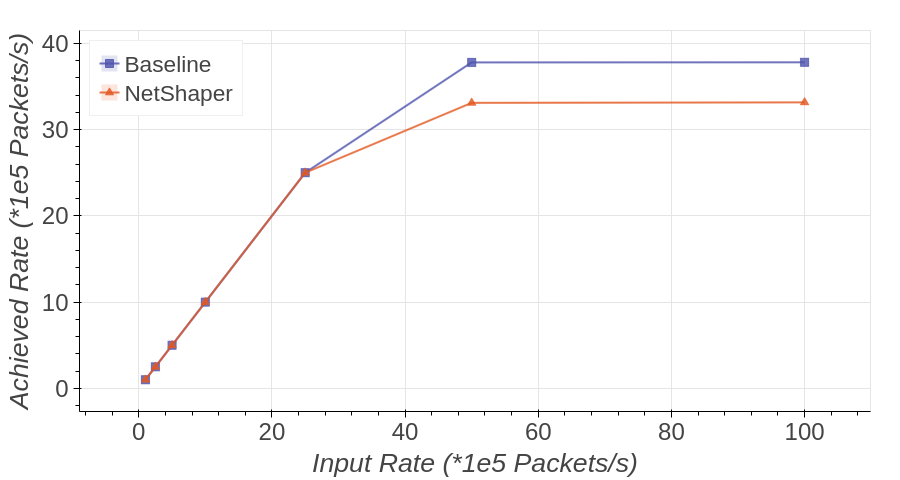
\includegraphics[width=\columnwidth]{figures/netshaper/evaluation/num_packets.png}
    \caption{Impact of NetShaper on transmitting small packets}
    \label{fig:netshaper-eval-num-packets}
\end{figure}